% !TeX root = ../main.tex

\chapter{Approach}\label{chapter:approach}
The purpose of the tool is the continuous detection of copied code in a changing codebase.
The work of Koschke et al. makes clear that a index based approach seems appropriate for continuous detection:
\glqq If the [copy-paste detection] analysis is to be conducted multiple times, creating an index pays off\grqq \cite{koschke2014large}.
Because of that, the tool is using an index to look up similar sections of code.
An index is a data structure which can be used to quickly look up values for a specific key.
For the index, a key-value store is used, which basically is a database representing a huge key-value map, where a key, e.g. a hash, points to a value.

This chapter describes the followed approach and architecture of the tool in detail.

\section{System Overview}
\begin{figure}[h]
	\centering
	\includegraphics{figures/architecture_overview.pdf}
	\caption{Tool Architecture Overview}\label{fig:tool_architecture}
\end{figure}
\autoref{fig:tool_architecture} shows an overview of the tool's client-server architecture.
The servers purpose is to provide a lookup service for similar code.
The client has a codebase which should be checked for license infringements.
It can use the server's service to find code in its codebase which is similar to code in open source systems.

The server has access to a pool of repositories and creates the index by normalizing and hashing files of the repositories as described in section \ref{section:approach/creating_index/normalization}.
Subsequently, the history of a reference system is analyzed as explained in section \ref{section:approach/creating_index/history_analysis}.
After that, the server generates a hash filter as described in section \ref{section:approach/creating_index/hash_filter}.

The client's search is two staged as described in \autoref{section:approach/searching_copied_code}
First the Scanner on the client normalizes and hashes code files in its codebase the same way the server does.
In the first stage, the Hash Filter is used to exclude hashes, which are not part of the server's index.
The Hash Filter can be downloaded from the server.
The second stage then requests the clone details from the server for the remaining hashes.
This can be done in a continuous manner, i.e. with every change on the client's codebase.

\section{Creating the Index}\label{section:approach/creating_index}
The index is based on the work of Hummel et al. \cite{hummel2010index}.
Source code files are considered as a list of statements.
Sequences of statements of a specific length - so called chunks - are compared by normalizing them, calculating the hash and then comparing the hash values.
Normalizing in this context means reducing the statements to parts of the code, which describe its structure and increase similarity as described in section \ref{section:approach/creating_index/normalization}.

To add a source code file to the index, it first is parsed and split into tokens.
A token represents a small part of the code such as a symbol, keyword, identifier, literal or comment.
The tokens then are normalized as described in section \ref{section:approach/creating_index/normalization}.
Now the tokens are aggregated into statements.
The tool then passes over the resulting list of statements using a sliding window to group together a chunk of code, which consists of several consecutive statements. %TODO image with indexing process

To reduce the space needed to store the information, which is required to identify similar code, chunks are hashed.
The hashes are then used as the key for the entry in the index.
The value of the entry is a list of locations, where chunks producing the hash can be found.
A client can then look for similar code by normalizing and calculating the hash of chunks the same way, as described in \autoref{section:approach/searching_copied_code}.
By looking up for the same hash in the index, locations of similar code can be found.

The amount of statements in a chunk influences the precision of a match, since longer chunks also require longer matches.
However, long chunks also reduces the probability to find chunks with modified, added or removed statements.
Therefore, the length of a chunk has to be short enough to find sequences of statements with modifications, but long enough, to exclude generic code, which would produce huge amounts of false positives. %TODO image?

\autoref{fig:normalization} shows the complete processing of an input file.

\subsection{Normalization}\label{section:approach/creating_index/normalization}
The normalization step removes irrelevant information and by that, concentrates on the essential features and properties of the code.
The level of similarity required for a match between two code segments can be adjusted by refining the level of normalization.
The parsing of code into tokens already does the first part of normalization by removing formatting.
After that, irrelevant tokens like access modifiers, import or include statements, comments or symbols like brackets or semicolons are removed.
The tokens which are left contain the main portion of information relevant for comparison of two sequences of code.

\subsection{History Analysis}\label{section:approach/creating_index/history_analysis}
It is important to also index old versions of the reference system, in order to detect code, which has been copied from older versions of an open source system.

To keep the index up to date and still keep information needed to find similarities with older versions of the file, changed files of reference systems are re-indexed.
For that, the server normalizes the new version of the file the same way as described before, groups it into chunks and hashes those chunks.
The resulting hashes are then inserted into the key value store.
If an entry for a hash already exists in the index, linking to a file with the same location, the old link is replaced with the new one to save space.
This ensures, that the entry for a chunk corresponding to a hash always points to the latest version of a file.
When files are deleted, nothing is changed in the key value store to keep the latest existing version of the file's chunk in the key-value store.

Instead of rescanning the whole file, only the chunks which have changed could be scanned.
However, the locations of hashes for chunks which did not change also have to be updated  in order to keep the latest version of a file in the index.

\subsection{Hash Filter}\label{section:approach/creating_index/hash_filter}
It is expected, that most of the calculated hashes of a target system can not be found in the index, since only small portions of code are copied.
Instead of sending a lookup-request for every hash to the server, a better option would be a local copy of the index for faster lookup and less load on the server.
However, the index is huge, since it may contain hashes and the according location for billions lines of code.
Distribution of the index to clients is a challenge, especially since the index has to be updated regularly.

With a table of all the hashes contained in the index, the client would be able to lookup whether a hash is in the index and only has to send a request to the server in this rare case.
This could significantly speed up the analysis, since only hashes which actually are in the index would be looked up.
On the server-side this also reduces the load.

Hashing with MD5 reduces the entropy of a chunk to about 128 bit of a ideal hash function, which still keeps the probability of collisions at a minimum.
Lossless compression is expected to reduce the size of the hashtable not by much, since randomness of hashes is very high.
However, lossy compression could be used.
One great way of reducing size of hash table with low false-positive probability is a BloomFilter.

To store a value, a BloomFilter uses multiple hash functions to hash a value \cite{bloom1970filter}.
It uses the resulting hash values as indexes to set bits of a bit array to 1.
To find out whether a value is stored in the BloomFilter, the value is hashed with the same hash functions as for storing a value.
Again, hash values are used as indexes.
If all values inside the bit array defined by the indexes are set to 1, the value is stored in the BloomFilter with a high probability.
If one or more of the bits are not set, the value is guaranteed not in the filter.
For the tool developed in this work, the values inserted into the BloomFilter are the hashes of the chunks.

The advantage here is the small size of the filter.
However, the compression is lossy, because there is a certain probability for false positives.
The probability is depending on the size of the bit array, the number of inserted values and the number of used hash functions, but when kept at an optimum, grows almost (due to discrete number of hashing functions) linearly with the number of insertions.
Since it is not possible to remove values from the filter, it has to be recalculated every time the index changes.

It is also possible to only use the filter to find code in a codebase with high probability of being copied.
This may be relevant for proprietary code with high confidentiality.
However, this does not allow the client to further investigate the code section and find the origin for a potential match automatically.
	
\section{Searching Copied Code}\label{section:approach/searching_copied_code}
The client has a codebase which should be searched for copied code.
To do so, it normalizes the code in question, groups statements and hashes them as described in \autoref{section:approach/creating_index}.
After that, the emerging hashes are filtered with the Bloom Filter.
Remaining hashes are then sent to the server, which responds with a map of hash to location for each hash.
As explained before, a hash may not be part of the index, but still pass the filter.
This false-positive can be recognized by the server and excluded from the response.

The response is then interpreted by the client.
By aggregating matches by reference system and file path, the relevance of the match can be assessed.

%TODO Activity diagram: client <-> server